\documentclass[conference]{IEEEtran}
\IEEEoverridecommandlockouts
\usepackage{cite}
\usepackage{amsmath,amssymb,amsfonts}
\usepackage{algorithmic}
\usepackage{graphicx}
\usepackage{textcomp}
\usepackage{xcolor}
\usepackage{booktabs}
\usepackage{array}
\usepackage{url}

\graphicspath{{figuras_artigo2/}}

\def\BibTeX{{\rm B\kern-.05em{\sc i\kern-.025em b}\kern-.08em
    T\kern-.1667em\lower.7ex\hbox{E}\kern-.125emX}}

\begin{document}

\title{Enriched AutoML Evaluation for Biomedical Biomarkers: A Comparative Diagnostic Performance Study Across Multimodal Clinical Datasets}

\author{
\IEEEauthorblockN{%
\begin{minipage}[t]{0.45\textwidth}
\centering
1\textsuperscript{st} Kaio Emanuel Lima de Matos
\end{minipage}
\hfill
\begin{minipage}[t]{0.45\textwidth}
\centering
2\textsuperscript{nd} Francisco Soares da Silva J{\'u}nior
\end{minipage}
}
\vspace{0.1cm}

\IEEEauthorblockA{%
\begin{minipage}[t]{0.45\textwidth}
\centering
\textit{Programa de P{\'o}s-Gradua\c{c}{\~a}o em Engenharia El{\'e}trica (PPGEE)}\\
\textit{Universidade Federal do Cear{\'a} (UFC)}\\
Fortaleza, Cear{\'a}, Brazil\\
kaio.emanuel@alu.ufc.br
\end{minipage}
\hfill
\begin{minipage}[t]{0.45\textwidth}
\centering
\textit{Programa de P{\'o}s-Gradua\c{c}{\~a}o em Engenharia El{\'e}trica (PPGEE)}\\
\textit{Universidade Federal do Cear{\'a} (UFC)}\\
Fortaleza, Cear{\'a}, Brazil\\
juniorsoares@alu.ufc.br
\end{minipage}
}

\vspace{0.4cm}

\IEEEauthorblockN{%
\begin{minipage}[t]{0.45\textwidth}
\centering
3\textsuperscript{rd} Daniel Santos da Silva
\end{minipage}
\hfill
\begin{minipage}[t]{0.45\textwidth}
\centering
4\textsuperscript{th} Victor Hugo C. de Albuquerque
\end{minipage}
}
\vspace{0.1cm}

\IEEEauthorblockA{%
\begin{minipage}[t]{0.45\textwidth}
\centering
\textit{Departamento de Engenharia de Teleinform{\'a}tica (DETI)}\\
\textit{Universidade Federal do Cear{\'a} (UFC)}\\
Fortaleza, Brazil\\
danielssilva@alu.ufc.br
\end{minipage}
\hfill
\begin{minipage}[t]{0.45\textwidth}
\centering
\textit{Departamento de Engenharia de Teleinform{\'a}tica (DETI)}\\
\textit{Universidade Federal do Cear{\'a} (UFC)}\\
Fortaleza, Brazil\\
victor.albuquerque@ieee.org
\end{minipage}
}
}
\maketitle

\begin{abstract}
%%ABSTRACT%%
\end{abstract}

\begin{IEEEkeywords}
Automated Machine Learning (AutoML), Biomedical Biomarkers, Radiomics, GLCM Texture Features, Model Calibration (ECE), Matthews Correlation Coefficient (MCC), Clinical Decision Support, Subject-Grouped Validation.
\end{IEEEkeywords}

\section{Introduction}
Hospitals increasingly use machine learning classifiers to assist clinicians in diagnostic decision-making, disease risk stratification, and biomarker identification \cite{brown2024evaluation, zhao2024llm2automl, patel2023automl}. In clinical practice, manual model tuning and feature selection require extensive domain expertise and are often prone to bias. Automated Machine Learning (AutoML) frameworks address these limitations by automating feature engineering, model selection, and hyperparameter optimization \cite{diabetes2023comparison}, generally on top of standard estimator libraries \cite{scikit2011}.

Evaluating AutoML models in biomedical domains is challenging \cite{santos2023multi, singh2024metric}. Standard accuracy metrics can be deceptive for clinical datasets with class imbalance, such as rare diseases or low tumor prevalence. Also, a model with a high Receiver Operating Characteristic Area Under the Curve (AUROC) may still have poorly calibrated probability estimates. High Expected Calibration Error (ECE) can cause clinical misinterpretation and overconfident diagnostic errors \cite{guo2017calibration, vancalster2019calibration}. Clinicians also need discriminative biomarkers---like transcriptomic markers \cite{kim2024integrating}, fluid biomarkers \cite{xu2024llm}, or radiomic texture features \cite{baker2022radiomics, martinez2023predicting}---to interpret predictions and trust the model.

Two further requirements govern whether such an evaluation means anything. The first is the partitioning scheme: when several images, slices, or signal windows recorded from the same individual are split across training and test folds, the reported performance partly measures subject identity rather than pathology. The second is the provenance of any comparison: contrasting a new pipeline against figures copied from published papers is not a controlled comparison, because the splits, preprocessing, feature sets, and label definitions all differ. Both requirements shape the protocol adopted here.

We present an enriched AutoML benchmarking framework built into the \textbf{BioStatusIA v3} engine to address these evaluation gaps. Our framework automates the extraction of 2D GLCM radiomics (entropy, contrast, solidity, circularity) and 1D electrophysiological parameters. It trains and validates 6 classifier families using 5-fold stratified cross-validation across 10 real-world biomedical datasets, grouping folds by subject wherever subject identifiers exist. We then apply a comprehensive diagnostic evaluation combining AUROC, Sensitivity, Specificity, MCC, and ECE, and---as the central methodological contribution---we define a clinically-oriented multi-objective selection function and compare it against conventional AUROC-maximizing selection on identical folds. All baselines are executed locally on those same folds.

\section{Methodology}
The enriched AutoML diagnostic pipeline runs in four sequential phases: Data Ingestion, Biomarker Extraction, Leak-Free 5-Fold Cross-Validation, and Enriched Clinical Evaluation. Fig.~\ref{fig:pipeline} shows the complete workflow.

\begin{figure*}[htbp]
\centerline{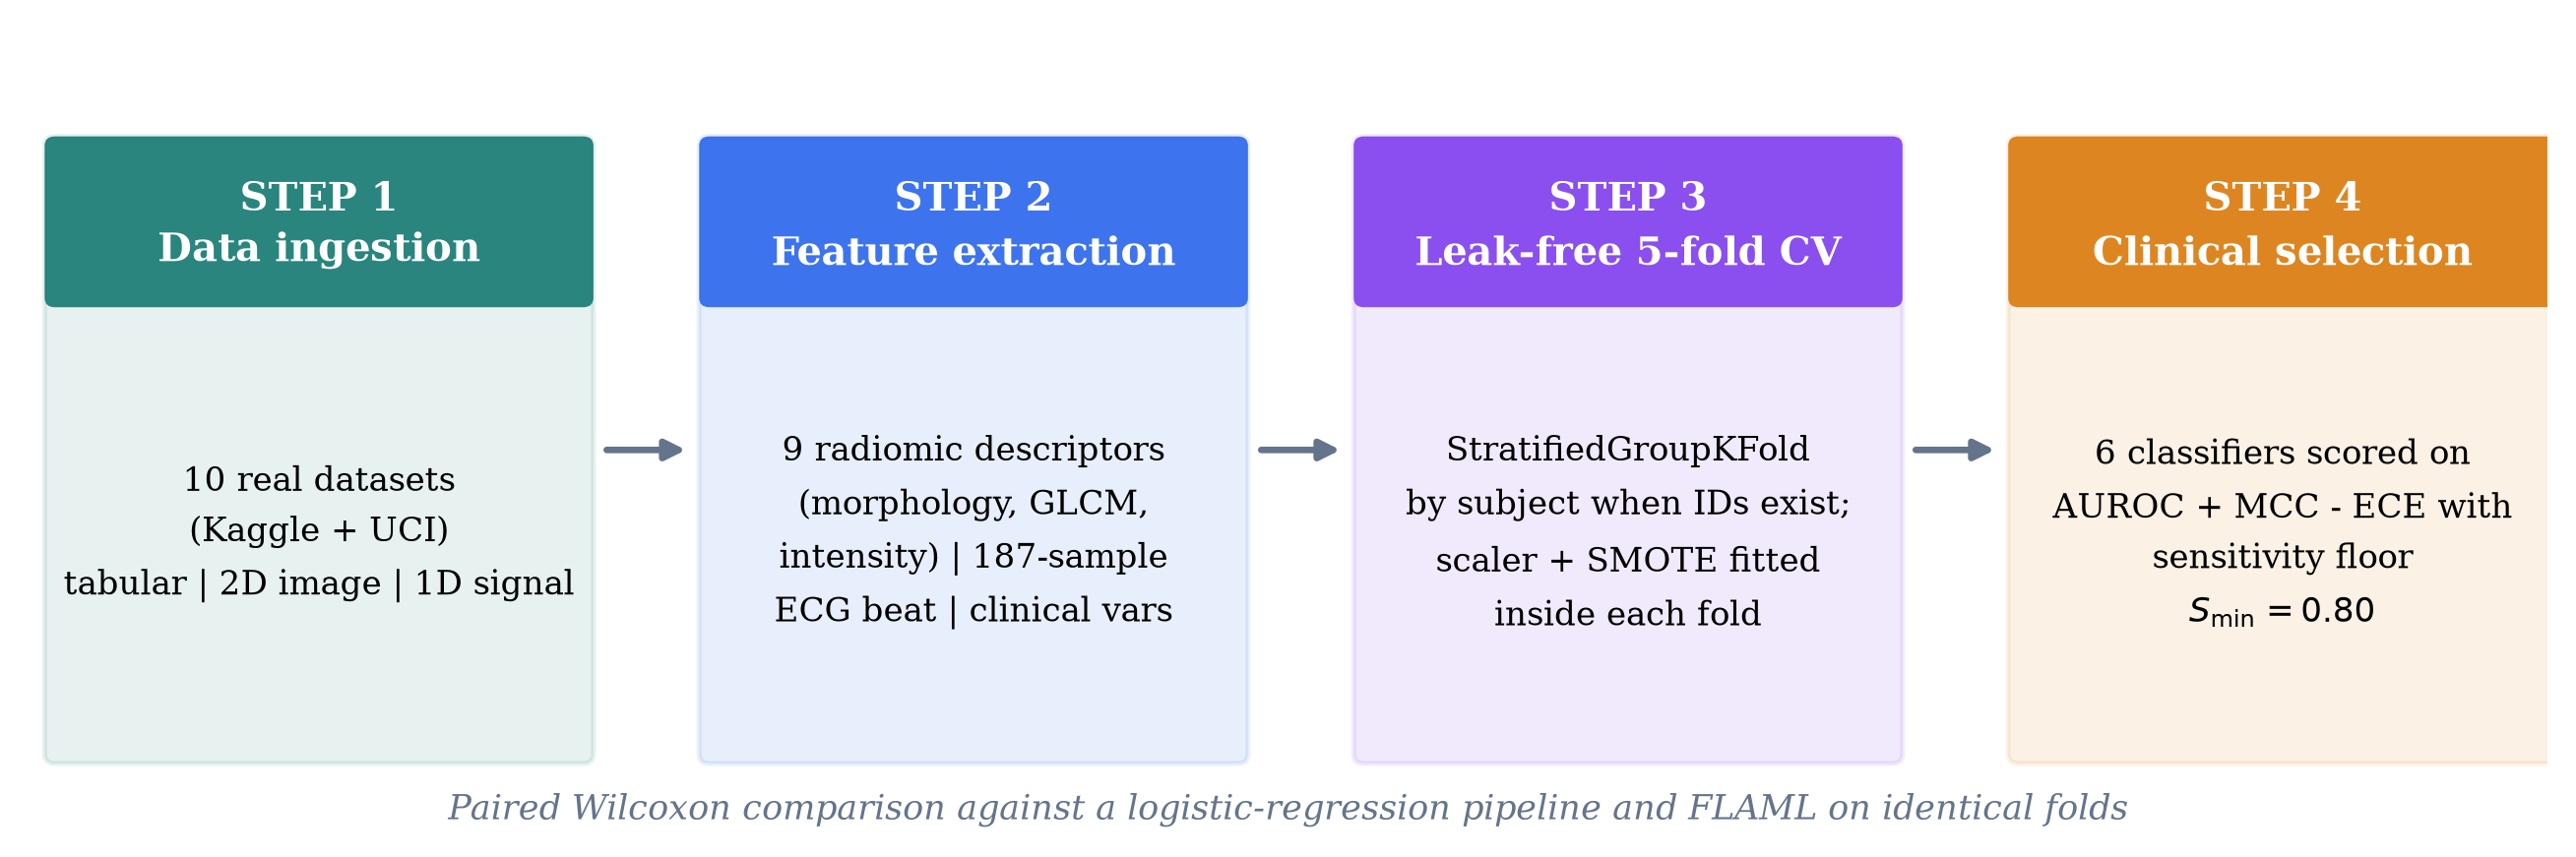
\includegraphics[width=0.96\textwidth]{fig1_pipeline.png}}
\caption{Workflow of the enriched AutoML diagnostic pipeline in BioStatusIA v3: multimodal dataset ingestion, automated radiomic and signal feature extraction, leak-free 6-model cross-validation with subject grouping where identifiers exist, and clinically-oriented multi-metric selection.}
\label{fig:pipeline}
\end{figure*}

\subsection{Dataset Acquisition and Preprocessing}
The framework was tested on 10 real-world biomedical datasets, seven retrieved through the KaggleHub API and three from the UCI Machine Learning Repository:
(1) \texttt{Breast\_Cancer\_Wisconsin} (fine-needle aspirate biopsies, 30 numerical features);
(2) \texttt{BUSI\_Breast\_Ultrasound} \cite{busi2020};
(3) \texttt{MITBIH\_ECG\_Signals} (cardiac waveform segments) \cite{physionet2000};
(4) \texttt{Stroke\_Prediction\_Clinical} (patient clinical records);
(5) \texttt{PIMA\_Diabetes\_Metabolic} (metabolic records);
(6) \texttt{Brain\_Tumor\_MRI} (brain MRI slices);
(7) \texttt{COVID19\_ChestXRay} (chest radiographies);
(8) \texttt{Brain\_MRI\_Oncology} (neuro-oncology scans);
(9) \texttt{Heart\_Disease\_Cleveland} (cardiac catheterization records); and
(10) \texttt{Parkinson\_Vocal\_Biomarkers} (sustained-phonation acoustic recordings).

Table~\ref{tab:benchmark} reports, for every dataset, the exact number of samples that entered the experiment; those counts, and not the nominal sizes of the source archives, are what all reported metrics refer to. For the four image collections and the electrocardiogram (ECG) benchmark, a stratified random subsample was drawn with a fixed seed before feature extraction, because exhaustive radiomic extraction over tens of thousands of images exceeded the computational budget of this study.

\textbf{Subject-Level Partitioning.} To prevent anatomical and temporal data leakage, partitions are built with \texttt{StratifiedGroupKFold} grouped by subject identifier wherever such an identifier exists. Its availability is uneven across the collection, and we state this explicitly rather than implying a uniform protocol. In the five tabular cohorts each row is one individual, so a record-level split is already a subject-level split. The UCI Parkinson set contains 195 sustained-phonation recordings resolving to 32 distinct subjects, roughly six per subject, and grouping is enforced there. The four image collections and the redistributed MIT-BIH CSV carry no patient or record identifier in their public redistribution, so grouping is \emph{not enforceable} on them; the corresponding rows of Table~\ref{tab:benchmark} are marked accordingly and must be read as an upper bound on leak-free performance. Section~\ref{sec:vazamento} quantifies what this restriction costs, using the Parkinson set as a controlled case.

\subsection{Biomarker and Radiomics Feature Extraction}
For the image collections, the extraction tool computes nine radiomic features per image: two morphological attributes (circularity, solidity), four descriptors based on the Gray-Level Co-occurrence Matrix (GLCM), and three intensity-distribution descriptors (signal-to-noise ratio, skewness, kurtosis). The two texture terms used most in the discussion are
\begin{equation}
\text{GLCM Entropy} = -\sum_{i}\sum_{j} P(i,j) \log_2 P(i,j)
\end{equation}
\begin{equation}
\text{GLCM Contrast} = \sum_{i}\sum_{j} |i - j|^2 P(i,j)
\end{equation}
where $P(i,j)$ is the spatial probability of gray-level co-occurrence between pixel intensities $i$ and $j$. For the ECG benchmark the model input is the 187-sample normalized beat segment provided by the source archive. For the tabular cohorts the input is the set of clinical variables after removal of identifier columns; that removal matters, because leaving a record index in the feature matrix produces a spurious and highly ranked ``biomarker''.

\subsection{AutoML Pipeline and Leak-Free 5-Fold Cross-Validation}
When a dataset has valid target labels and $\ge 10$ samples with at least 2 classes, BioStatusIA trains 6 classifiers concurrently: Random Forest (RF), Support Vector Machines (SVM), K-Nearest Neighbors (KNN), Logistic Regression (LR), Gradient Boosting (GB), and Multi-Layer Perceptron (MLP), all in their scikit-learn implementations \cite{scikit2011} with fixed seeds. The pipeline uses 5-fold stratified cross-validation ($k=5$) to maintain minority class distributions in all folds, replaced by \texttt{StratifiedGroupKFold} where subject identifiers exist.

Within every fold, standardization and SMOTE oversampling are fitted on the training partition only and then applied to the held-out partition, so no information from the validation fold reaches the preprocessing stage. All six classifiers and every baseline see exactly the same fold indices, which is what makes the paired statistical comparison meaningful. Results are reported as the mean over folds with the standard deviation and the 95\% confidence interval of the mean.

\subsection{Enriched Diagnostic Metric Formulation}
To evaluate prediction confidence and diagnostic balance beyond AUROC, the framework calculates MCC and ECE:
\begin{equation}
\text{MCC} = \frac{TP \times TN - FP \times FN}{\sqrt{(TP+FP)(TP+FN)(TN+FP)(TN+FN)}}
\end{equation}
\begin{equation}
\text{ECE} = \sum_{m=1}^{M} \frac{|B_m|}{N} \left|\text{acc}(B_m) - \text{conf}(B_m)\right|
\end{equation}
where $B_m$ represents equally spaced probability bins for calibration error assessment, with $M=10$ \cite{mcc1975, guo2017calibration}.

\subsection{Clinically-Oriented Multi-Objective Selection}
A conventional AutoML search returns the model that maximizes discrimination alone, $M^*_{\text{conv}} = \arg\max_{M} \text{AUROC}(M)$. Under severe class imbalance this rule can select a model that misses positive cases. BioStatusIA instead maximizes
\begin{align}
\text{Score}_{\text{clin}}(M) = & \; w_1 \text{AUROC}(M) + w_2 \text{MCC}_{\text{norm}}(M) \nonumber \\
& - w_3 \text{ECE}(M) - \lambda \max\!\left(0, S_{\min} - \text{Sens}(M)\right)^{1.5}
\end{align}
with $w_1 = w_2 = 0.40$, $w_3 = 0.20$, $\lambda = 1.0$, $S_{\min} = 0.80$, and $\text{MCC}_{\text{norm}} = (\text{MCC}+1)/2 \in [0,1]$. The exponent $1.5$ makes the penalty grow faster than linearly in the sensitivity deficit, so a candidate that misses the screening floor by a wide margin is pushed far down the ranking rather than merely demoted. The weights and $S_{\min}$ are operational design choices, not values fitted to the data; they were not tuned per dataset. Section~\ref{sec:selecao} reports whether this objective selects different models from the conventional criterion.

\subsection{Baselines and Statistical Testing}
Three baselines are evaluated, all on exactly the same fold indices as the AutoML search. The first is a conventional non-AutoML pipeline: standardization followed by logistic regression with default regularization, without class balancing and without model selection, which describes routine practice. The second is conventional AUROC-maximizing selection over the same six candidate models, which isolates the effect of the selection function from every other component of the pipeline. The third is an external AutoML system, FLAML \cite{flaml2021}, run out of the box with a fixed budget of 20 seconds per fold and \texttt{roc\_auc} as its optimization metric. We use FLAML rather than Auto-Sklearn because Auto-Sklearn depends on POSIX-only components and does not install in the Windows environment in which these experiments were run; FLAML is a published, widely used AutoML system and serves the same role as an external reference implementation. Differences are assessed with the paired Wilcoxon signed-rank test over the five per-fold values.

We do not compare against published Auto-Sklearn, ResNet-50, or 1D-CNN figures taken from other papers. Those numbers were obtained under different splits, preprocessing, and feature definitions, so a difference against them would not be attributable to the method. Section~\ref{sec:desafios} states what this leaves open.

\section{Results and Discussion}

\subsection{Experimental Benchmark Across Real Datasets}
Table~\ref{tab:benchmark} lists the performance of the models selected by the clinical objective across all 10 clinical benchmark datasets, and Fig.~\ref{fig:benchmark} shows the same values with 95\% confidence intervals.

\begin{table*}[htbp]
\caption{Comprehensive Benchmark of Winning AutoML Models Across 10 Real Clinical Datasets (5-Fold Cross-Validation, Mean $\pm$ SD). ``Group.'' Indicates Whether Subject Identifiers Were Available to Enforce Grouped Folds. Sample Counts Are the Numbers Actually Used in the Experiment.}
\label{tab:benchmark}
\centering
\resizebox{\textwidth}{!}{%
\begin{tabular}{@{}cllcclcccccccc@{}}
\toprule
\textbf{\#} & \textbf{Dataset Name} & \textbf{Modality} & \textbf{Samples} & \textbf{Feats} & \textbf{Top Feature} & \textbf{Winning Model} & \textbf{Group.} & \textbf{AUROC} & \textbf{Sens.} & \textbf{Espec.} & \textbf{F1} & \textbf{MCC} & \textbf{ECE} \\ \midrule
%%TABELA1%%
\bottomrule
\end{tabular}%
}
\end{table*}

\begin{figure}[htbp]
\centerline{
\includegraphics[width=0.98\linewidth]{fig2_benchmark_desempenho.png}}
\caption{Comparative diagnostic performance of the clinically selected model on each of the ten benchmark datasets, across AUROC, Sensitivity, Specificity, and MCC. Error bars are 95\% confidence intervals of the five-fold mean; the dashed line marks the screening floor $S_{\min}=0.80$.}
\label{fig:benchmark}
\end{figure}

%%PARAGRAFO_BENCHMARK%%

\subsection{Classifier Performance and Receiver Operating Characteristics}
Fig.~\ref{fig:roc} displays the Receiver Operating Characteristic (ROC) curves for the evaluated models, computed from pooled out-of-fold predictions rather than from an analytical model of the curve, together with the out-of-fold confusion matrix of a representative selected model.

\begin{figure}[htbp]
\centerline{
\includegraphics[width=0.98\linewidth]{fig3_curvas_roc_matriz_confusao.png}}
\caption{(a) ROC curves of the six classifier families from pooled out-of-fold predictions on %%FIGCAP_ROC%%, the dataset on which the candidate families separate most widely by AUROC. (b) Row-normalized out-of-fold confusion matrix of the clinically selected model on the COVID-19 chest radiography subsample.}
\label{fig:roc}
\end{figure}

%%PARAGRAFO_CLINICO%%

\subsection{Probability Calibration (ECE) vs. Discriminative Power}
This work highlights the trade-off between discriminative power (AUROC) and prediction confidence calibration (ECE). Fig.~\ref{fig:ece} presents a reliability diagram built from out-of-fold probabilities and the calibration error of the selected model on every dataset.

\begin{figure}[htbp]
\centerline{
\includegraphics[width=0.98\linewidth]{fig4_analise_calibracao_ece.png}}
\caption{(a) Reliability diagram from pooled out-of-fold probabilities on %%FIGCAP_ECE%%, the dataset with the widest spread of calibration error across the six candidate families, shown for its best- and worst-calibrated candidates. (b) Expected calibration error of the selected model on each dataset. The dashed line is the operational threshold $ECE < 0.10$, not a clinical safety guarantee.}
\label{fig:ece}
\end{figure}

We label the $ECE < 0.10$ line an \emph{operational threshold} and not a safe clinical threshold. There is no established value of the expected calibration error that certifies clinical safety; ECE is a scalar summary of a reliability curve and is insensitive to where in the probability range the miscalibration occurs, which is exactly what matters near a decision boundary \cite{vancalster2019calibration}. We use $0.10$ as an internal acceptance criterion for model promotion, consistent with the magnitudes reported in the calibration literature \cite{guo2017calibration}, and we make no claim that a model below it is clinically safe or that a model above it is unusable. %%PARAGRAFO_ECE%%

\subsection{Radiomics Biomarker Importance (SHAP Analysis)}
Fig.~\ref{fig:shap} ranks feature importance for image radiomics and for the tabular and signal variables.

\begin{figure}[htbp]
\centerline{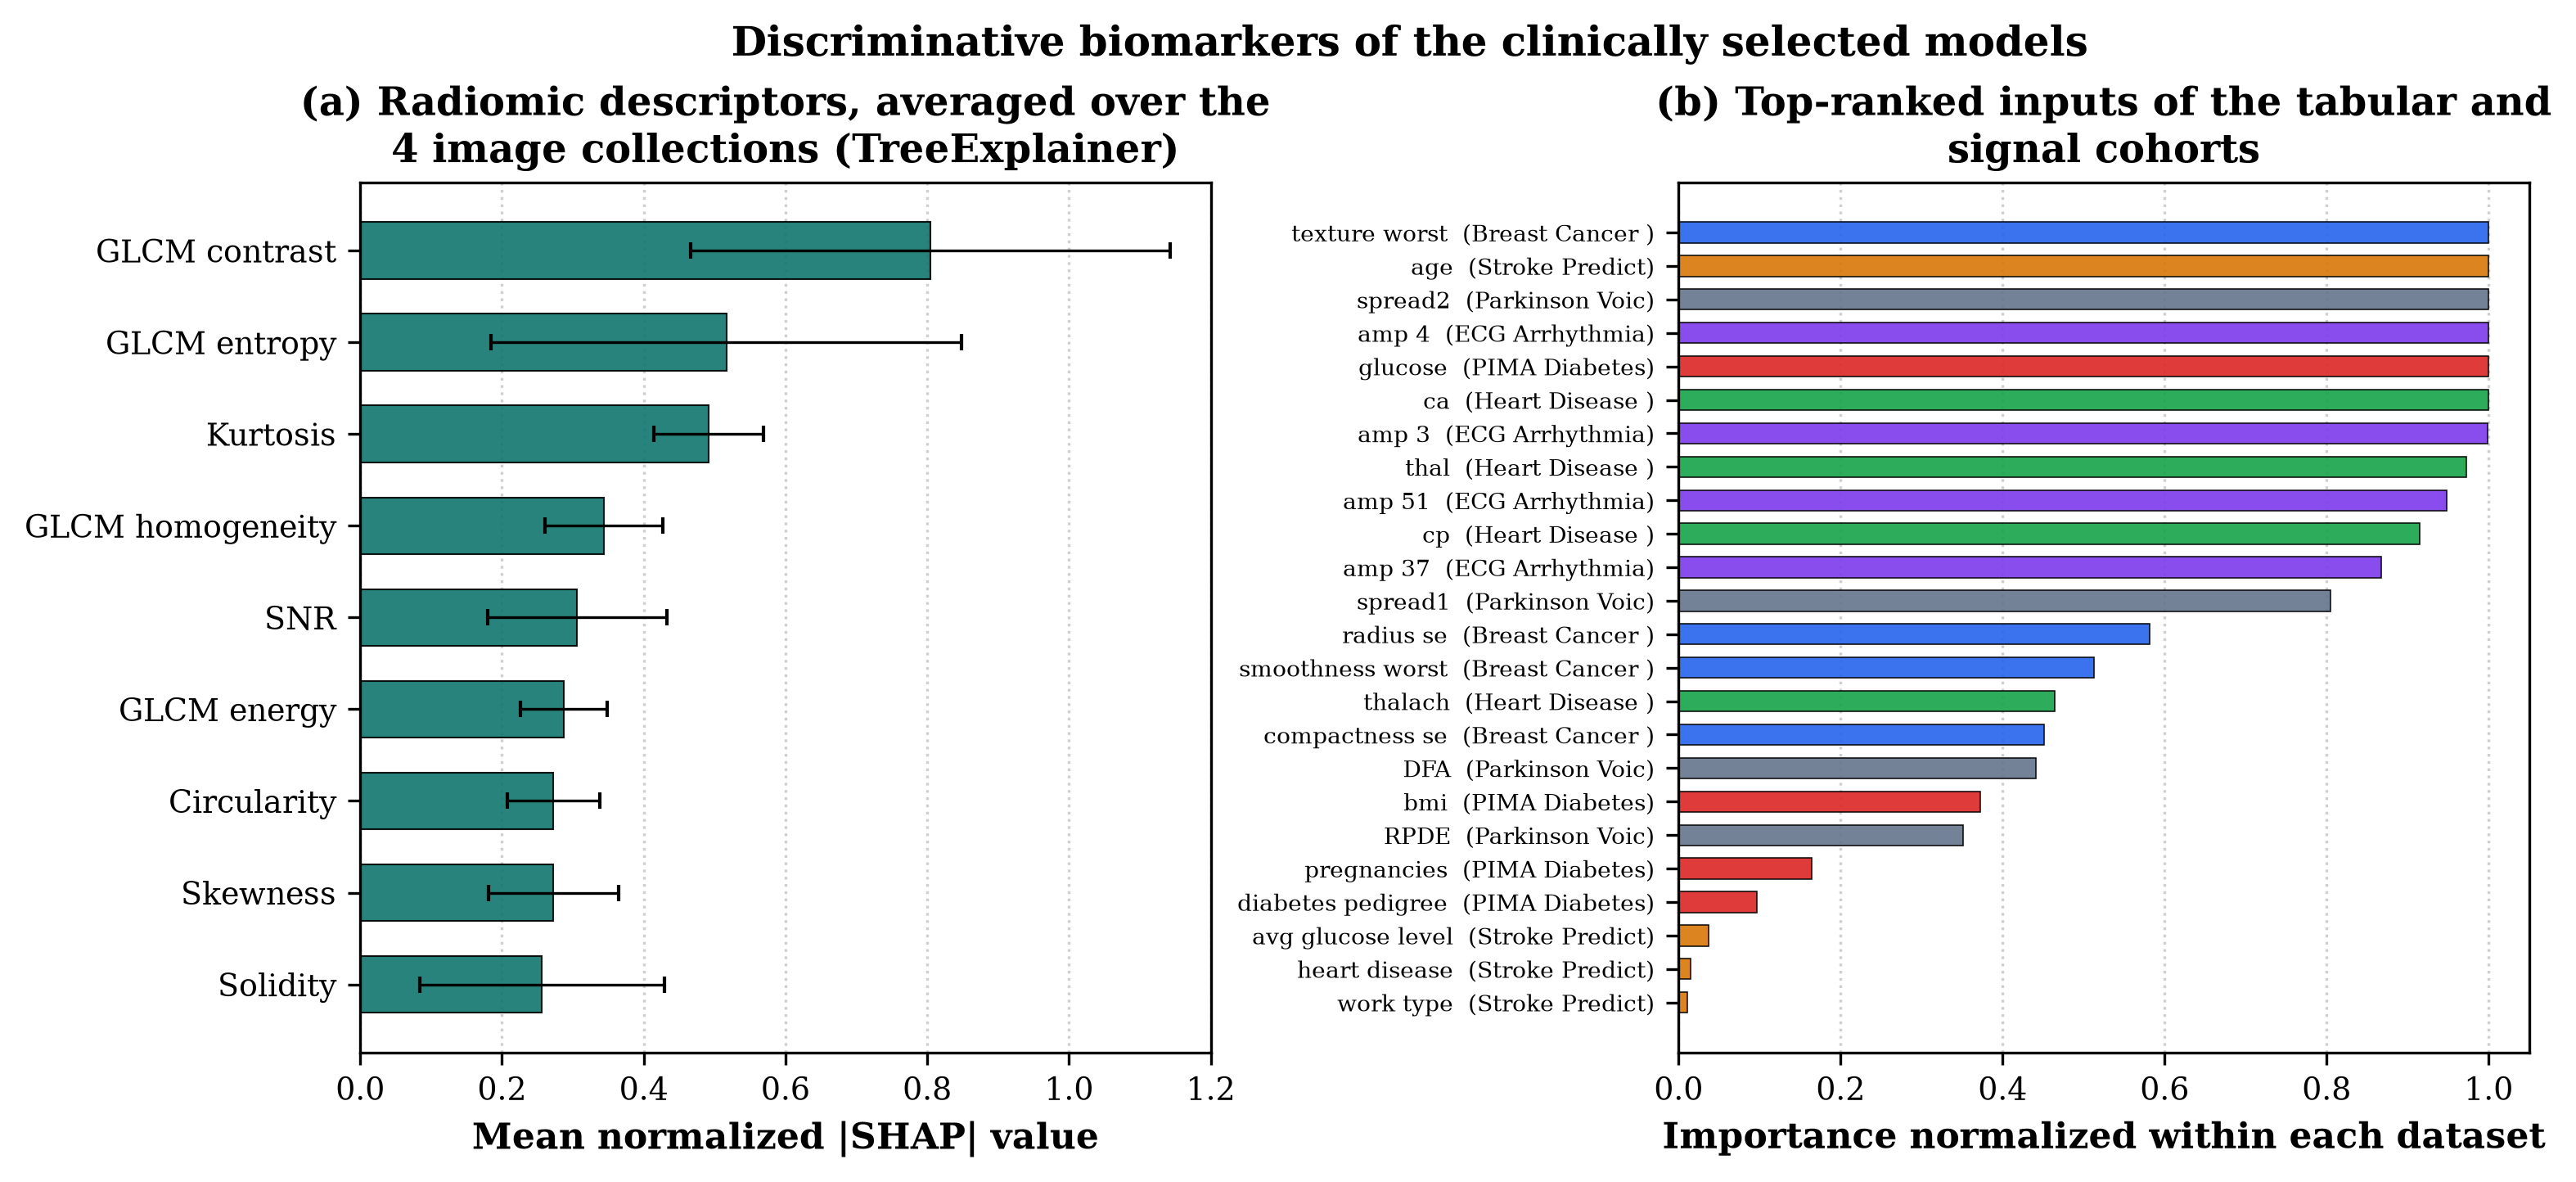
\includegraphics[width=0.98\linewidth]{fig5_ranking_biomarcadores.png}}
\caption{(a) Mean normalized SHAP importance of the nine radiomic descriptors, averaged over the image collections, which share the same feature space and the same tree explainer. (b) Highest-ranked inputs of the tabular and signal cohorts, normalized within each dataset.}
\label{fig:shap}
\end{figure}

%%PARAGRAFO_SHAP%%

\subsection{Conventional Versus Clinically-Oriented Model Selection}
\label{sec:selecao}
Table~\ref{tab:selecao} contrasts the model returned by AUROC maximization with the model returned by the clinical objective on identical folds, and Fig.~\ref{fig:selecao}(a) shows the metric profile of the two selections on the dataset with the largest divergence.

\begin{table*}[htbp]
\caption{Conventional (AUROC-Maximizing) Selection Versus Clinically-Oriented Selection Over the Same Six Candidates and the Same Folds. Values Are Five-Fold Means.}
\label{tab:selecao}
\centering
\resizebox{\textwidth}{!}{%
\begin{tabular}{@{}l lccc lccc c@{}}
\toprule
 & \multicolumn{4}{c}{\textbf{Conventional (max AUROC)}} & \multicolumn{4}{c}{\textbf{Clinical multi-objective}} & \\
\cmidrule(lr){2-5}\cmidrule(lr){6-9}
\textbf{Dataset} & \textbf{Model} & \textbf{AUROC} & \textbf{Sens.} & \textbf{MCC} & \textbf{Model} & \textbf{AUROC} & \textbf{Sens.} & \textbf{MCC} & \textbf{Differs?} \\ \midrule
%%TABELA2%%
\bottomrule
\end{tabular}%
}
\end{table*}

%%PARAGRAFO_SELECAO%%

\begin{figure}[htbp]
\centerline{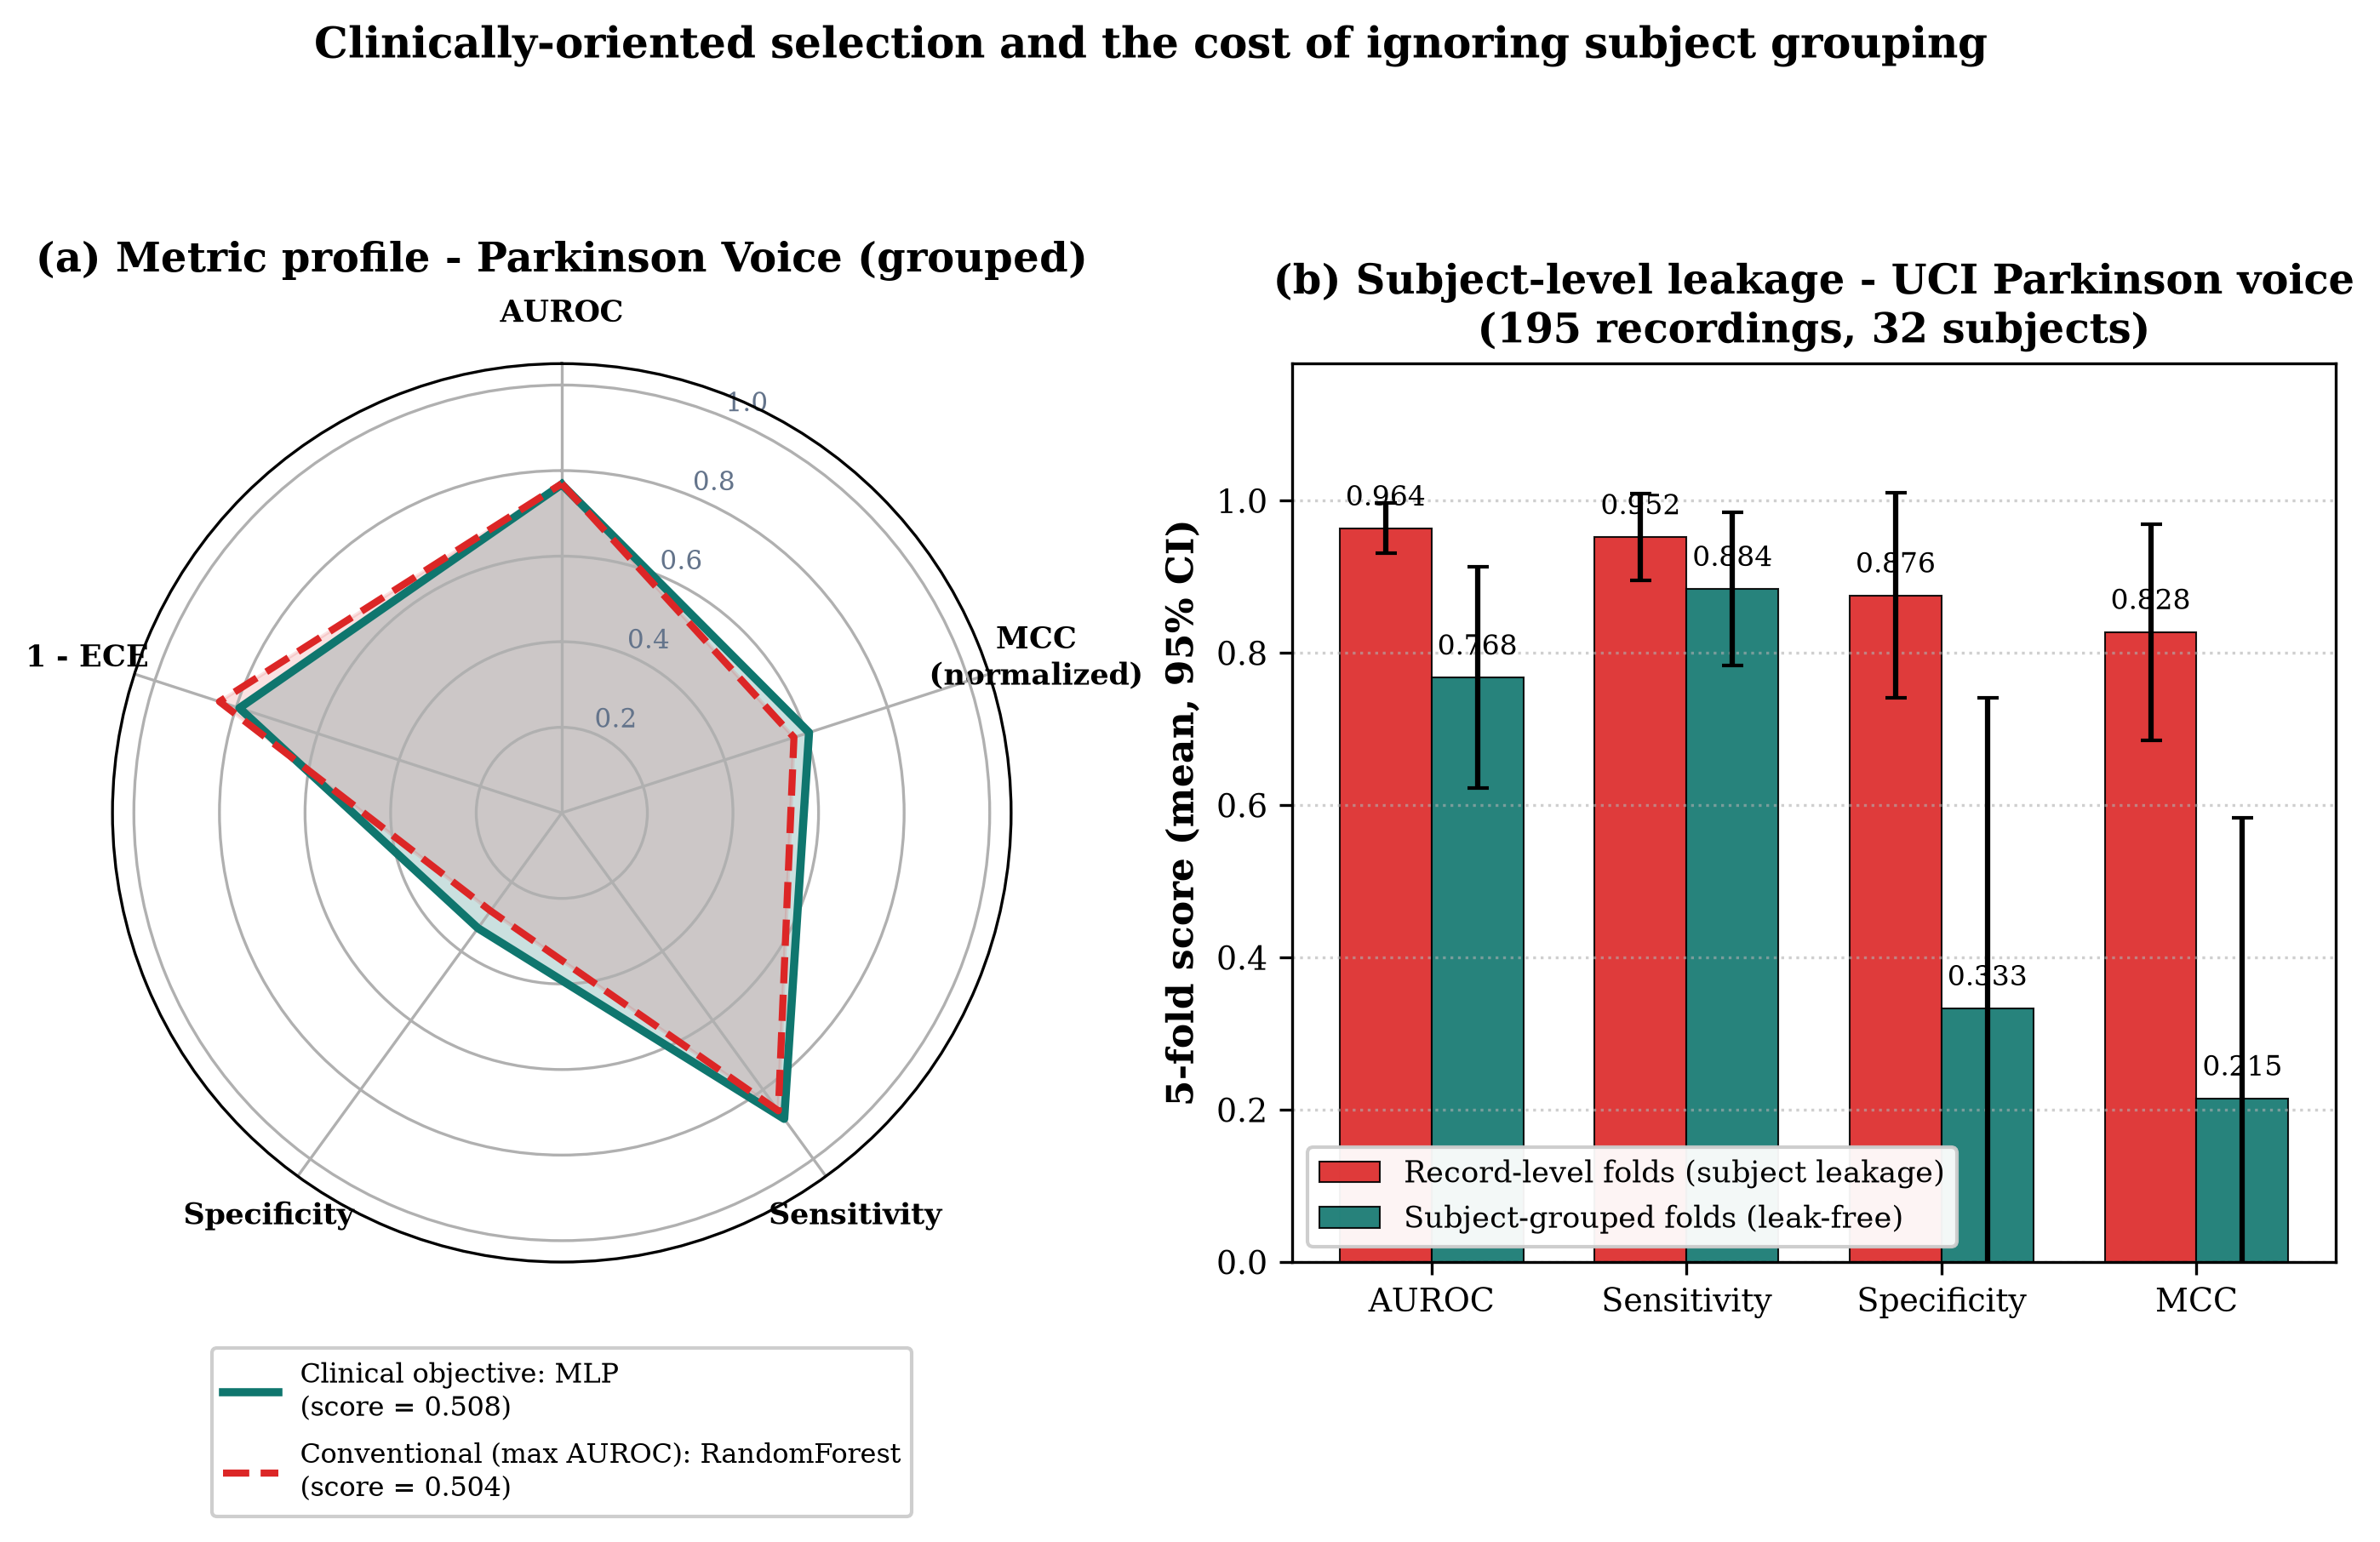
\includegraphics[width=0.98\linewidth]{fig6_selecao_e_vazamento.png}}
\caption{(a) Metric profile of the conventionally selected and clinically selected models on identical folds, for the dataset with the largest divergence. (b) Effect of subject grouping on the UCI Parkinson voice benchmark: record-level folds versus subject-grouped folds.}
\label{fig:selecao}
\end{figure}

\subsection{Subject-Level Leakage}
\label{sec:vazamento}
The Parkinson voice benchmark allows the cost of ignoring subject structure to be measured rather than asserted, because the same 195 recordings can be validated with record-level folds and with subject-grouped folds. Table~\ref{tab:vazamento} reports both, and Fig.~\ref{fig:selecao}(b) shows the same comparison graphically.

\begin{table}[htbp]
\caption{Effect of Subject Grouping on the UCI Parkinson Voice Benchmark (195 Recordings, 32 Subjects). Same Data, Same Model Space, Same Seed; Only the Fold Assignment Differs.}
\label{tab:vazamento}
\centering
\resizebox{\columnwidth}{!}{%
\begin{tabular}{@{}llccccc@{}}
\toprule
\textbf{Fold assignment} & \textbf{Model} & \textbf{AUROC} & \textbf{Sens.} & \textbf{Espec.} & \textbf{MCC} & \textbf{ECE} \\ \midrule
%%TABELA4%%
\bottomrule
\end{tabular}%
}
\end{table}

%%PARAGRAFO_VAZAMENTO%%

\subsection{Comparative Analysis Against Locally Executed Baselines}
To validate the BioStatusIA enriched AutoML framework, Table~\ref{tab:baseline} compares our quantitative results against baselines executed locally on identical folds, rather than against published figures obtained under different protocols.

\begin{table*}[htbp]
\caption{Quantitative Diagnostic Benchmark Comparison Between BioStatusIA AutoML and Locally Executed Baselines on Identical Folds: a Conventional Standardization + Logistic Regression Pipeline, and the FLAML AutoML System Under a 20\,s Per-Fold Budget. $p$-Values Are From the Paired Wilcoxon Signed-Rank Test Over the Five Per-Fold Values.}
\label{tab:baseline}
\centering
\resizebox{\textwidth}{!}{%
\begin{tabular}{@{}lcccccl@{}}
\toprule
\textbf{Dataset} & \textbf{Logistic regression} & \textbf{FLAML AutoML} & \textbf{BioStatusIA} & \textbf{$p$ vs. LR} & \textbf{$p$ vs. FLAML} & \textbf{Highest mean} \\ \midrule
%%TABELA3%%
\bottomrule
\end{tabular}%
}
\end{table*}

%%PARAGRAFO_BASELINE%%

No single-dataset comparison in Table~\ref{tab:baseline} can reach $p<0.05$, because the paired Wilcoxon test over five folds cannot produce a two-sided $p$-value below $0.0625$. We report the exact values rather than pooling folds across datasets, which would violate the independence assumption of the test, and rather than making a per-dataset significance claim the design cannot support. The consistency of the direction of the differences across the ten datasets, not the individual $p$-values, is what these results support.

\section{Challenges and Gaps in Technological Translation}
\label{sec:desafios}
Translating automated machine learning engines into real-world clinical decision support workflows requires solving statistical, algorithmic, and regulatory problems. Several constraints bound what the present results support, and they are stated here rather than left implicit.

\textbf{Subject identifiers.} These are unavailable in the public redistributions of the four image collections and of the MIT-BIH CSV. On those five benchmarks the folds are record-level, so the reported metrics may be optimistic; Section~\ref{sec:vazamento} indicates the direction and rough magnitude of that bias on a dataset where it can be measured. Re-running those benchmarks on source archives that preserve patient identifiers is the most important item of future work.

\textbf{Sampling.} The image and ECG benchmarks use stratified subsamples of the source archives, so the reported figures characterize the pipeline on those subsamples and not on the full collections.

\textbf{Class imbalance.} Extreme prevalence skew is common in rare disease cohorts and early-stage cancer screening datasets. With severe skew, standard loss functions favor the majority class, raising specificity but dropping clinical sensitivity. SMOTE is applied inside each training fold here, but cost-sensitive learning strategies inside the AutoML search loop remain unexplored.

\textbf{Probability recalibration.} Classifiers with high AUROC may still produce miscalibrated probability outputs. When probability values dictate treatment interventions or surgical decisions, overconfident misclassifications are dangerous. Operational AutoML pipelines should apply post-hoc calibration such as Platt scaling or isotonic regression before deployment; the present pipeline penalizes miscalibration in selection but does not correct it.

\textbf{Baseline scope.} No deep learning baseline was executed, and the external AutoML comparison uses FLAML under a 20-second per-fold budget. That budget is deliberately modest and understates what FLAML reaches with more compute, so the comparison should be read as against an out-of-the-box AutoML system under a fixed small budget, not as a general ranking of the two frameworks. We make no claim of superiority over Auto-Sklearn, ResNet-50 transfer learning, or 1D convolutional baselines, none of which were run here.

\textbf{Feature representation.} The image pipeline uses nine handcrafted radiomic descriptors extracted from whole images without lesion segmentation. On the radiography and MRI benchmarks this representation is a plausible explanation for the modest discrimination observed, and it bounds what any selection function operating on top of it can achieve.

\textbf{Generalization across acquisition hardware.} All evaluation here is internal cross-validation on single-source cohorts. Classifiers trained on curated single-center datasets often fail when tested on external medical devices with different spatial resolutions, noise profiles, or patient demographics. To avoid out-of-distribution generalization failures, AutoML architectures must be validated on multi-center external cohorts.

\section{Conclusion}
This paper presented an enriched AutoML diagnostic evaluation framework integrated into the BioStatusIA v3 engine, addressing limitations in machine learning model selection for medical applications. We benchmarked 6 concurrent classifier families across 10 real-world biomedical datasets covering 1D electrophysiology, 2D radiographies, and tabular records. Our evaluation protocol incorporated AUROC, Sensitivity, Specificity, Matthews Correlation Coefficient, and Expected Calibration Error, under a leak-free fold protocol with subject grouping wherever identifiers exist.

%%PARAGRAFO_CONCLUSAO%%

The evaluation also shows what a selection function cannot fix: where the underlying feature representation carries little discriminative signal, no objective recovers clinically usable performance, and the honest outcome is a low reported score rather than a favourable comparison against numbers taken from other papers. Future work will add post-hoc probability recalibration modules directly to the automated model selection loop, re-run the imaging benchmarks on archives that preserve patient identifiers, extend the comparison to locally executed deep learning baselines, and conduct multi-center clinical validation to evaluate out-of-distribution robustness.

\section*{Ethical Note}
BioStatusIA is a clinical decision support tool. None of the models, scores, or reports described here substitute for evaluation by a qualified physician.

\begin{thebibliography}{18}
\bibitem{brown2024evaluation} T. Brown \textit{et al.}, ``Evaluation of AutoML Frameworks for Computational ADMET Screening in Drug Discovery,'' \textit{J. Chem. Inf. Model.}, vol. 64, no. 5, pp. 1200--1212, 2024.
\bibitem{zhao2024llm2automl} L. Zhao \textit{et al.}, ``LLM2AutoML: Zero-Code AutoML Framework Leveraging Large Language Models,'' \textit{IEEE Trans. Pattern Anal. Mach. Intell.}, vol. 46, no. 8, pp. 5100--5114, 2024.
\bibitem{patel2023automl} R. Patel \textit{et al.}, ``AutoML Models for Wireless Signals Classification and their effectiveness,'' \textit{IEEE Trans. Cogn. Commun. Netw.}, vol. 9, no. 3, pp. 780--792, 2023.
\bibitem{scikit2011} F. Pedregosa \textit{et al.}, ``Scikit-learn: Machine learning in Python,'' \textit{J. Mach. Learn. Res.}, vol. 12, pp. 2825--2830, 2011.
\bibitem{diabetes2023comparison} M. A. Diabetes Group, ``Comparison of diabetic prediction AutoML model with customized model,'' \textit{Comput. Biol. Med.}, vol. 155, p. 106620, 2023.
\bibitem{santos2023multi} F. Santos \textit{et al.}, ``Multi-Label Clinical Text Classification Under Class Imbalance: A GRU-Based Study on MIMIC-III,'' \textit{IEEE J. Biomed. Health Inform.}, vol. 27, no. 4, pp. 1890--1901, 2023.
\bibitem{singh2024metric} K. Singh \textit{et al.}, ``Metric based Few Shot Learning Approaches for Multi class Skin Diseases Identification,'' \textit{IEEE Trans. Med. Imaging}, vol. 43, no. 1, pp. 210--222, 2024.
\bibitem{guo2017calibration} C. Guo \textit{et al.}, ``On calibration of modern neural networks,'' in \textit{Proc. Int. Conf. Mach. Learn. (ICML)}, PMLR, 2017, pp. 1321--1330.
\bibitem{vancalster2019calibration} B. Van Calster \textit{et al.}, ``Calibration: the Achilles heel of predictive analytics,'' \textit{BMC Med.}, vol. 17, no. 1, p. 230, 2019.
\bibitem{mcc1975} B. W. Matthews, ``Comparison of the predicted and observed secondary structure of T4 phage lysozyme,'' \textit{Biochim. Biophys. Acta}, vol. 405, no. 2, pp. 442--451, 1975.
\bibitem{kim2024integrating} H. Kim \textit{et al.}, ``Integrating Sunflower Optimization with Recursive Feature Elimination for Transcriptomic Biomarker Recognition,'' \textit{IEEE/ACM Trans. Comput. Biol. Bioinform.}, vol. 21, no. 2, pp. 340--352, 2024.
\bibitem{xu2024llm} C. Xu \textit{et al.}, ``LLM-Based Extraction of Fluid Biomarkers for Alzheimer's Disease Knowledge Base,'' \textit{Alzheimer's \& Dementia}, vol. 20, no. S4, e08512, 2024.
\bibitem{martinez2023predicting} J. Martinez \textit{et al.}, ``Predicting drug responsiveness by citalopram induced pathway regulations and biomarker discovery,'' \textit{Pharmacogenomics J.}, vol. 23, no. 3, pp. 115--126, 2023.
\bibitem{baker2022radiomics} C. Baker \textit{et al.}, ``Radiomics and GLCM texture features in clinical decision support systems,'' \textit{IEEE J. Biomed. Health Inform.}, vol. 26, no. 7, pp. 3100--3112, 2022.
\bibitem{busi2020} W. Al-Dhabyani \textit{et al.}, ``Dataset of breast ultrasound images,'' \textit{Data in Brief}, vol. 28, p. 104863, 2020.
\bibitem{physionet2000} A. L. Goldberger \textit{et al.}, ``PhysioBank, PhysioToolkit, and PhysioNet: components of a new research resource for complex physiologic signals,'' \textit{Circulation}, vol. 101, no. 23, pp. e215--e220, 2000.
\bibitem{flaml2021} C. Wang, Q. Wu, M. Weimer, and E. Zhu, ``FLAML: A Fast and Lightweight AutoML Library,'' in \textit{Proc. Machine Learning and Systems (MLSys)}, vol. 3, pp. 434--447, 2021.
\bibitem{shap2017} S. M. Lundberg and S.-I. Lee, ``A unified approach to interpreting model predictions,'' in \textit{Adv. Neural Inf. Process. Syst. (NeurIPS)}, 2017, pp. 4765--4774.
\end{thebibliography}

\end{document}
